% !TeX root = ../../main.tex
% Add the above to each chapter to make compiling the PDF easier in some editors.

\chapter{Background and Foundations}\label{chapter:background_and_foundations}

This chapter represents the basic concepts used throughout our work. First, a brief introduction to the reinforcement learning field. Second, Markov Decision Processes (MDPs), the standard mathematical formalism framework for reinforcement learning will be introduced. Then, We will discuss the value functions and policy gradient methods. Next, we will discuss the methods used to achieve the RL goal and differentiate between them. In addition, we conclude the use of deep learning in reinforcement learning with some of Deep Reinforcement Learning (DRL) Algorithms. Finally, we discuss related work in distributed reinforcement learning.

\section{Reinforcement Learning}

\textbf{RL} (\textit{The science of decision making}) is a machine learning approach to teach agent how to solve tasks through trial and error interaction with a dynamic, unknown environment. It formalizes the idea of \textit{\textbf{rewarding or punishing}} an agent for its behavior. This makes the agent more likely to repeat or forego that behavior in the future. In contrast with other machine learning methods, the agent is not told the proper actions to take. Instead, the agent interacts with its environment, and upon observing the consequences of its actions, it can learn to alter its behavior in response to rewards received. The goal of the agent is to maximize the expected cumulative reward. The main components of RL are the \textbf{Agent} and the \textbf{Environment}. The typical interaction loop between agent and environment is illustrated in Figure~\ref{fig:agent_env} below.

\begin{figure}[!htb]
	\centering
	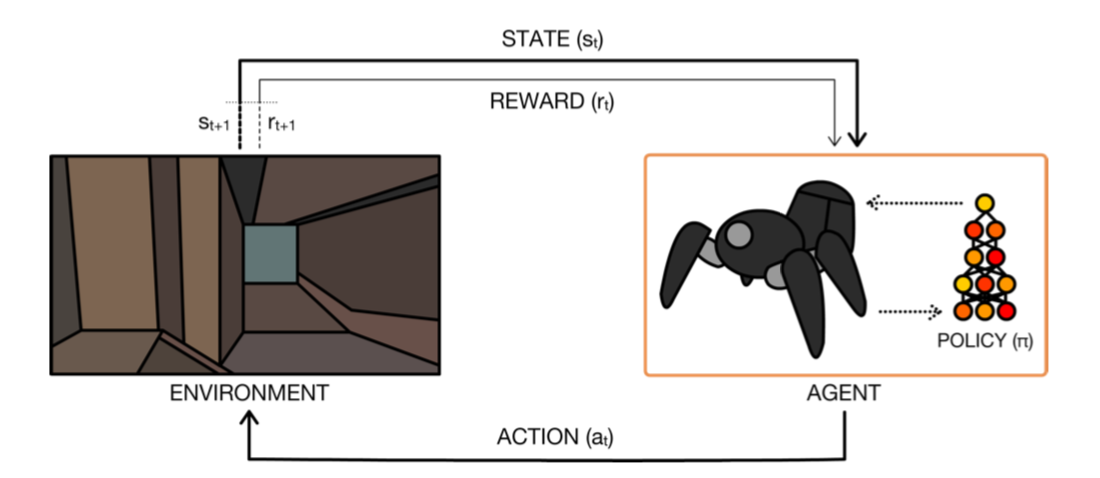
\includegraphics[width=.5\linewidth]{figures/Agent-Env.png}
	\caption{Reinforcement Learning interaction loop. The agent takes an action at a\textsubscript{t} state s\textsubscript{t}. The environment then responds with the corresponding reward r\textsubscript{t+1} and the new state s\textsubscript{t+1}, which are fed back to the agent~\parencite{arulkumaran2017brief}}
	\label{fig:agent_env}
\end{figure}

\subsubsection{Agent}\label{Agent}

An agent is considered the brain (e.g. for a robot, the agent is typically not the whole robot, but the specific program running on the robot's CPU that makes the decision on the action). The agent decides to takes proper actions and it is where the learning process happen and improve over time. For the learning process, the agent observes the state of the world and based on that takes an action. The environment changes according to the agent's actions and it might also change on its own. Examples of the agents are a drone making a delivery, or a robot learning to walk.
%or super mario navigating a video game. 

\subsubsection{Environment}\label{Environment}

An Environment constitutes a world for the agent to act and learn from. To describe the environment to an agent we have a \textbf{state} \(s\) which is a complete description of the state of the world. Sometimes an \textbf{observation} \(o\) is a \textit{partial} description of a state, which may omit information. Environments could be the whole surrounding 3D space or 2D images from cameras for a real-world task like a robotic arm, or it could represent an entire virtual world or games from an emulator like OpenAI Gym~\parencite{brockman2016openai}. When the agent can observe the complete state of the environment, we say that the environment is \textbf{fully observed} (e.g. Atari games). When the agent can only see a partial observation, we say that the environment is \textbf{partially observed} (e.g. robotic camera in a navigation task).
Some of the environments can be found in this figure~\ref{fig:envs_examples}

% !TeX root = ../../main.tex

\begin{figure}[h!]
		\centering
		\begin{subfigure}[b]{0.3\textwidth}
				\centering
				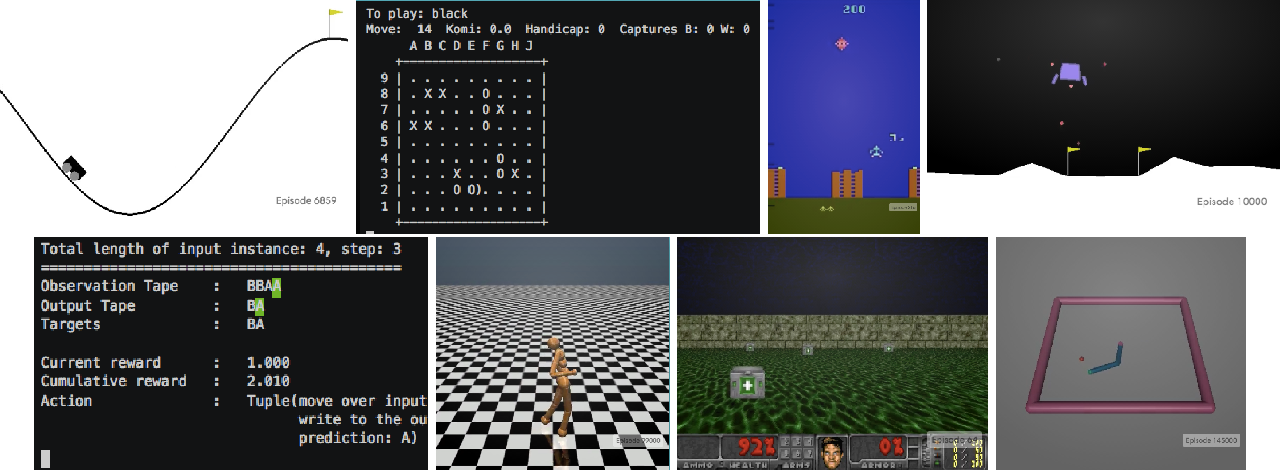
\includegraphics[width=0.7\textwidth]{figures/existing_envs/openai_gym}
				\caption{OpenAI Gym}
				\label{fig:openai_gym}
		\end{subfigure}
		\hfill
		\begin{subfigure}[b]{0.3\textwidth}
				\centering
				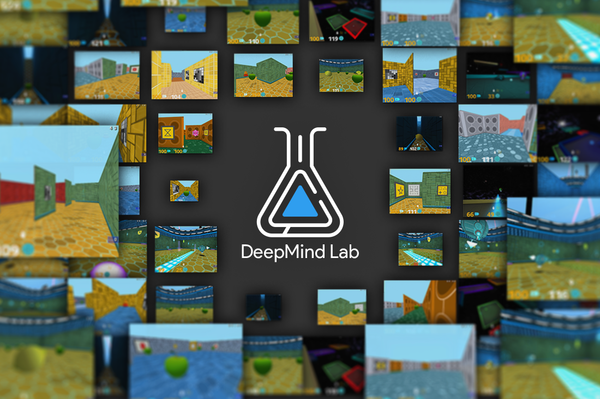
\includegraphics[width=0.7\textwidth]{figures/existing_envs/deepmind_lab.png}
				\caption{DeepMind Lab}
				\label{fig:deepmind_lab}
		\end{subfigure}
		\hfill
		\begin{subfigure}[b]{0.3\textwidth}
				\centering
				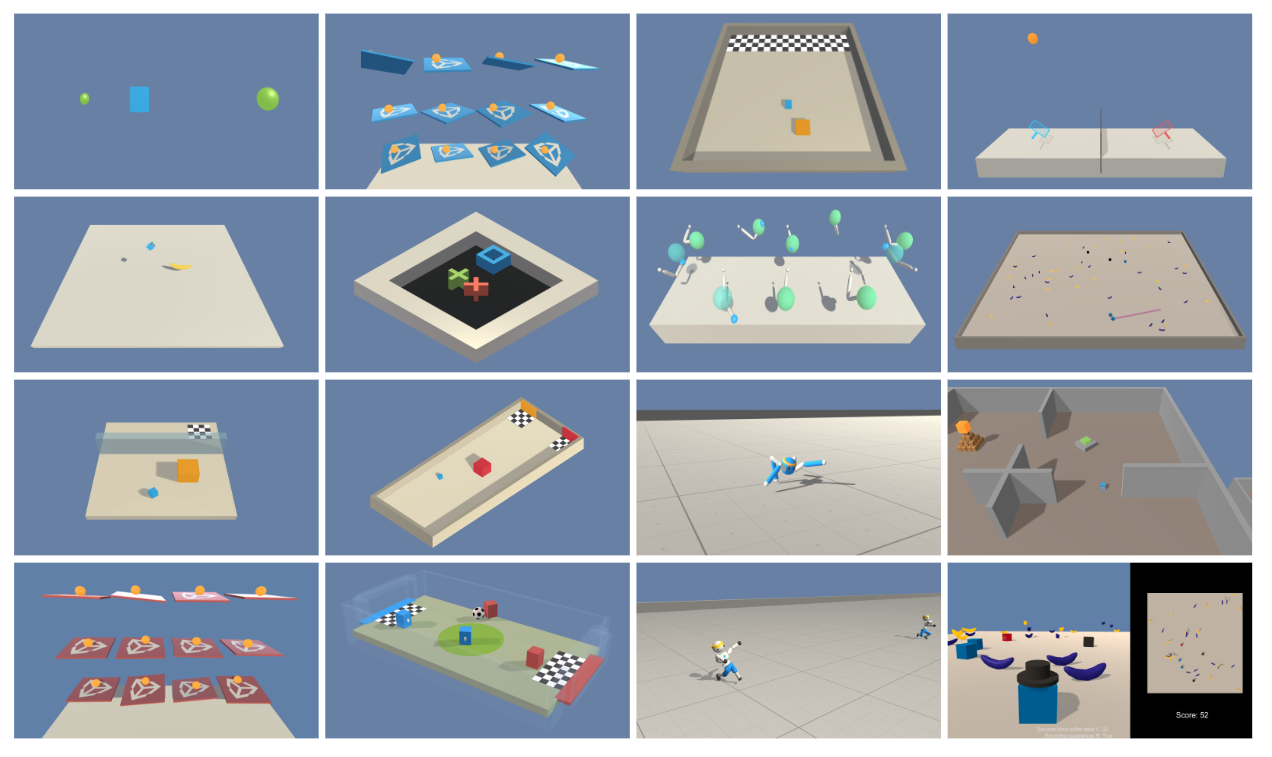
\includegraphics[width=0.7\textwidth]{figures/existing_envs/unity_mlagents.png}
				\caption{Unity MLAgents}
				\label{fig:unity_mlagents}
		\end{subfigure}
		\hfill

		\begin{subfigure}[b]{0.3\textwidth}
				\centering
				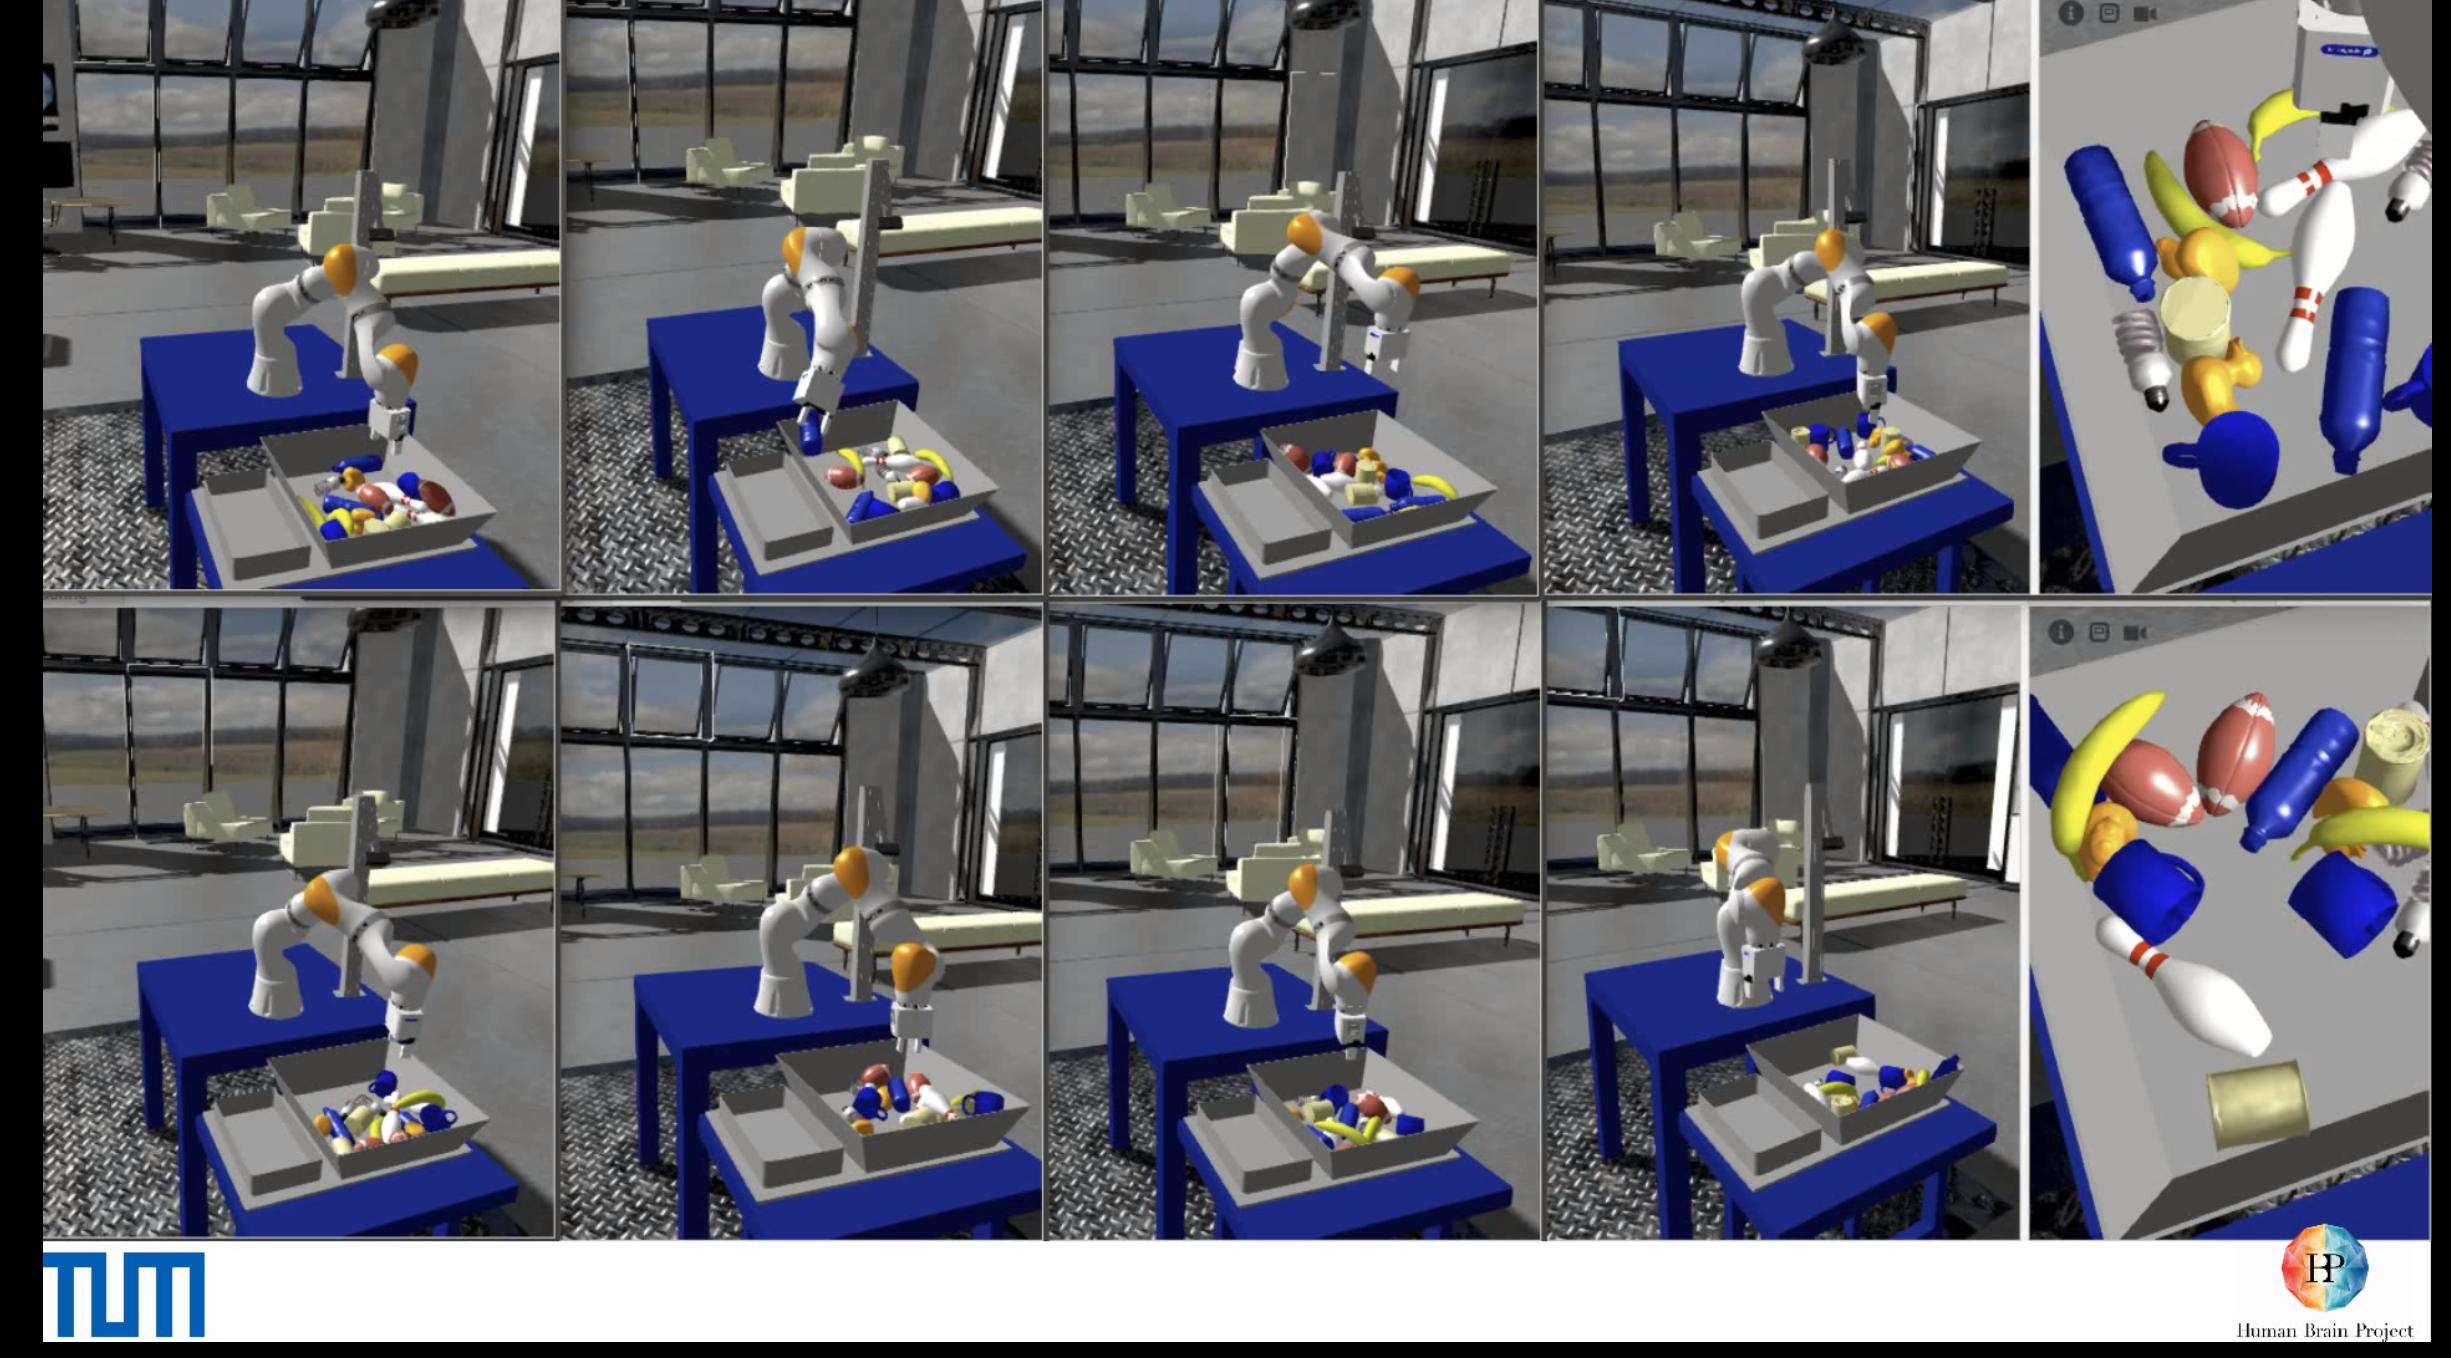
\includegraphics[width=0.7\textwidth]{figures/existing_envs/nrp.png}
				\caption{Neurorobotics Platform}
				\label{fig:atari_2600}
		\end{subfigure}
		\hfill
		\begin{subfigure}[b]{0.3\textwidth}
				\centering
				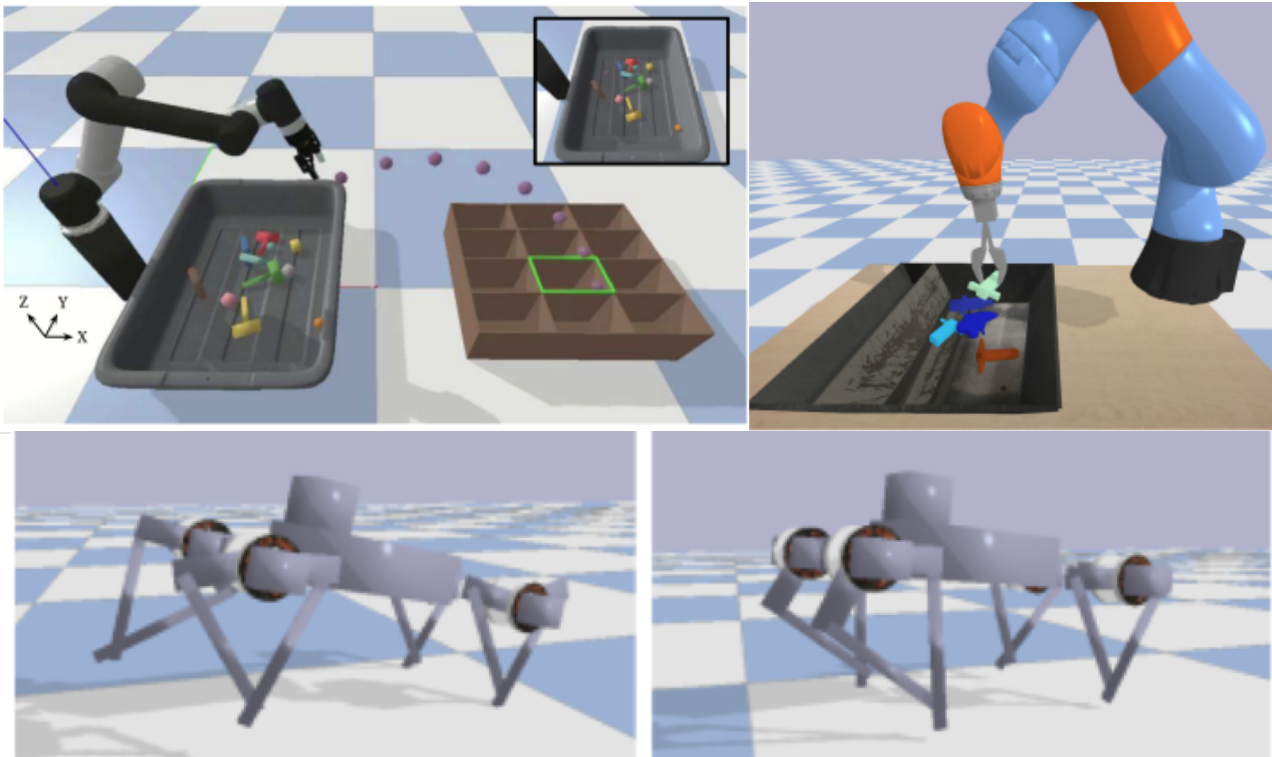
\includegraphics[width=0.7\textwidth]{figures/existing_envs/pybullet.png}
				\caption{PyBullet}
				\label{fig:pybullet}
		\end{subfigure}
		\hfill
		\begin{subfigure}[b]{0.3\textwidth}
				\centering
				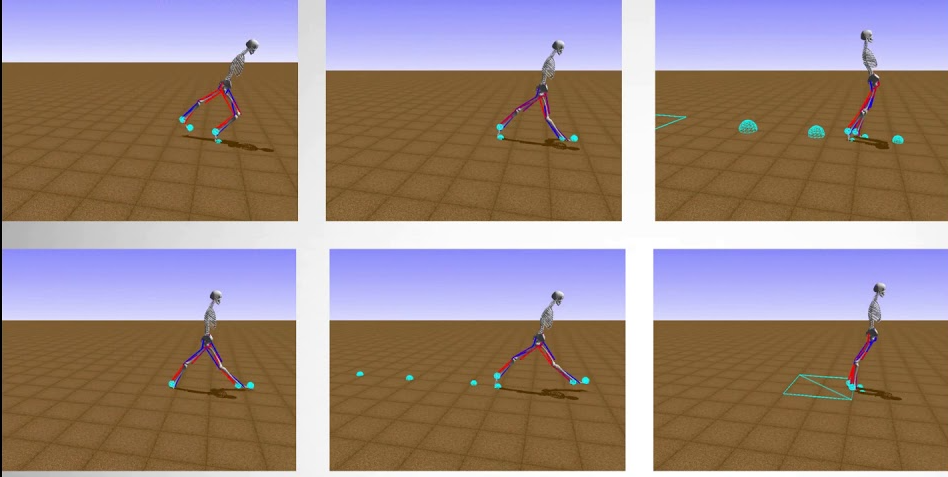
\includegraphics[width=0.7\textwidth]{figures/existing_envs/osim_rl.png}
				\caption{Osim RL: musculoskeletal models in OpenSim}
				\label{fig:osim_rl}
		\end{subfigure}

		\begin{subfigure}[b]{0.3\textwidth}
				\centering
				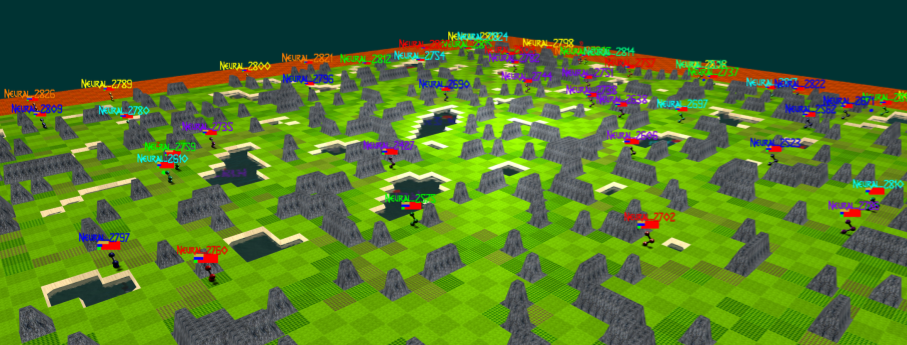
\includegraphics[width=0.7\textwidth]{figures/existing_envs/openai_mmo.png}
				\caption{OpenAI MML}
				\label{fig:openai_mmo}
		\end{subfigure}
		\hfill
		\begin{subfigure}[b]{0.3\textwidth}
				\centering
				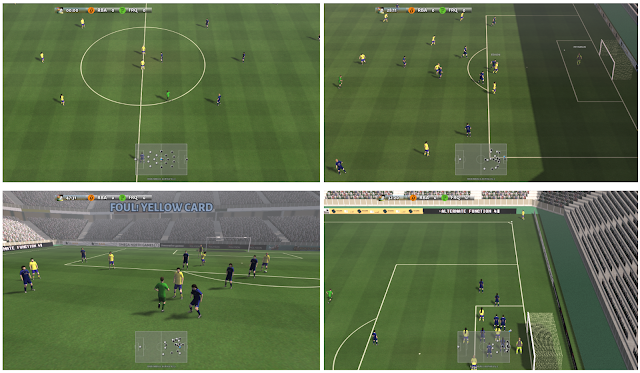
\includegraphics[width=0.7\textwidth]{figures/existing_envs/google_football.png}
				\caption{Google Research Football}
				\label{fig:google_football}
		\end{subfigure}
		\hfill
		\begin{subfigure}[b]{0.3\textwidth}
				\centering
				\includegraphics[width=0.7\textwidth]{figures/existing_envs/deepmind_alphstar.png}
				\caption{StarCraft II Learning Environment}
				\label{fig:deepmind_alphstar}
		\end{subfigure}
	\hfill
		 \caption{Examples of existing Deep RL Environments}
		 \label{fig:envs_examples}
\end{figure}

\subsection{Markov Decision Process}

Formally, reinforcement learning can be described as a Markov decision process, An MDP is a 5-tuple, $ \left\langle S, A, \mathcal{T}, R, \gamma \right\rangle $ which consists of:

\begin{itemize}
	\item A set of all states \(S\), plus a distribution of starting states \(p(s0)\).
	\item A set of valid actions \(A\).
	\item Transition dynamics $ \mathcal{T}\left(\mathbf{s}_{t+1} | \mathbf{s}_{t}, \mathbf{a}_{t}\right) $ that map a state-action pair at time \(t\) onto a distribution of states at time \(t+1\).
	\item An immediate $ \mathcal{R}\left(\mathbf{s}_{t}, \mathbf{a}_{t}, \mathbf{s}_{t+1}\right) $ reward function.
	\item A discount factor \(\gamma \in(0,1)\), where lower values place more emphasis on immediate rewards.
\end{itemize}

Extra objects can be defined depending on problem setting:
\begin{itemize}
	\item $\rho_0$: Initial state distribution
\end{itemize}

Markov Decision Process refers to the fact that the system obeys the \textbf{Markov property}: which indicates that transitions only depend on the most recent state and action, and no prior history, in other words, the future is conditionally independent of the past given the present state. $ p\left(s_{t+1} | s_{1}, a_{1}, \ldots, s_{t}, a_{t}\right)=p\left(s_{t+1} | s_{t}, a_{t}\right) $


\subsection{Rewards and Return}

The reward function (\(R\)) is critically important in RL. It depends on the current state of the world, the action just taken, and the next state of the world:

\begin{center}
	\begin{equation}
		r_{t}=R\left(s_{t}, a_{t}, s_{t+1}\right).
	\end{equation}
\end{center}

The goal of the agent is to maximize some notion of cumulative reward over a trajectory. There are two kinds of return, \textbf{the finite-horizon undiscounted return}, which is just the sum of rewards obtained in a fixed window of steps:

\begin{center}
	\begin{equation} \label{eq:1}
		R(\tau)=\sum_{t=0}^{T} r_{t}.
	\end{equation}
\end{center}

Another kind of return is \textbf{the infinite-horizon discounted return}, which is the sum of all rewards ever obtained by the agent, but \textit{discounted} by how far off in the future they’re obtained. This formulation of reward includes a discount factor \(\gamma \in(0,1)\):

\begin{center}
	\begin{equation} \label{eq:2}
		R(\tau)=\sum_{t=0}^{\infty} \gamma^{t} r_{t}.
	\end{equation}
\end{center}

The use of a discount factor is crucial as \textbf{mathematically} an infinite-horizon sum of rewards may not converge to a finite value, and is hard to deal with in equations. But with a discount factor and under reasonable conditions, the infinite sum converges.

\subsection{Policies}

A policy ($\pi$) is a rule used by an agent to decide what actions to take. It's considered as the strategy that the agent employs to determine the next action based on the current state. It maps states to actions $ \pi : \mathcal{S} \rightarrow p(\mathcal{A}=\mathbf{a} | \mathcal{S}) $, the actions that promise the highest reward.

The policy can be deterministic where it is usually denoted by $ \mu: a_{t}=\mu\left(s_{t}\right) $ or stochastic denoted by $ \pi:  a_{t} \sim \pi\left(\cdot | s_{t}\right) $
with the two most common kinds of stochastic policies categorical policies (discrete action spaces) and diagonal Gaussian policies (continuous action spaces).

A very important two key computations for training stochastic policies are:
\begin{itemize}
	\item Sampling actions from the policy, and
	\item Computing log likelihoods of particular actions, $ \log \pi_{\theta}(a|s) $.
\end{itemize}


\subsubsection{Reinforcement Learning Goal}

The goal of RL is to select a policy which maximizes the \textbf{expected return} ($ J(\pi) $) when the agent acts according to it, where:
\begin{center}
	\begin{equation} \label{eq:expected_return}
		J(\pi)=\int_{\tau} P(\tau | \pi) R(\tau)=\underset{\tau \sim \pi}{\mathrm{E}}[R(\tau)],
	\end{equation}
\end{center}

with $ P(\tau | \pi) $ as the probability distributions over \textit{T-step} trajectories.
\begin{center}
	\begin{equation}
		P(\tau | \pi)=\rho_{0}\left(s_{0}\right) \prod_{t=0}^{T-1} P\left(s_{t+1} | s_{t}, a_{t}\right) \pi\left(a_{t} | s_{t}\right).
	\end{equation}
\end{center}

So the central optimization problem of reinforcement learning can be described as:
\begin{center}
	\begin{equation}
		\pi^{*}=\arg \max _{\pi} J(\pi),
	\end{equation}
\end{center}
with $\pi^*$ being the optimal policy.


\subsection{Learning Optimal Policies}

There are two main approaches to solve reinforcement learning problems: methods based on \textit{value functions} (Critic-only), and methods based on \textit{policy search} (Actor-only). There is also a hybrid, \textit{actor-critic approach}, which combines both value functions and policy search, where the actor and critic are both represented explicitly and learned separately. We will now explain these approaches and other useful concepts for solving RL problems.

\subsubsection{Critic-only: Learning based on value functions}
Critic only methods are based on the idea to first find the optimal value function and then to derive an optimal policy from this value function.  Value function methods are based on estimating the value (expected return) of being in a given state. The state-value function $V^{\pi}(\mathbf{s})$ is the expected return when starting in state $\mathbf{s}$ and following $\pi$ is defined as:
\begin{center}
	        \begin{equation}
	                V^{\pi}(\mathbf{s})=\mathbb{E}[R | \mathbf{s}, \pi],
	        \end{equation}
\end{center}

and the optimal state-value function defined as:
\begin{center}
	        \begin{equation}
	                V^{*}(\mathbf{s})=\max _{\pi} V^{\pi}(\mathbf{s}) \quad \forall \mathbf{s} \in \mathcal{S}.
	        \end{equation}
\end{center}

The optimal policy, $\pi^{*}$, has a corresponding state-value function $V^{*}(\mathbf{s})$ where it could be retrieved by choosing among all actions available at $\mathbf{s_t}$ and picking the action $\mathbf{a}$ that maximizes expected optimal value for the succeeding state.

In practice, the MDP is often unknown and the transition dynamics $\mathcal{T}$ are unavailable so the only way to get information about it is by interacting with the environment and observing rewards.
Hence, construct another function, the \textit{state-action value or quality function} $Q^{\pi}(\mathbf{s}, \mathbf{a})$ estimates the value function and derives an optimal policy. 
It is similar to $V^{\pi}$, except that the initial action $\mathbf{a}$ is provided, and $\pi$ is only followed from the succeeding state onwards:
\begin{center}
	        \begin{equation}
	                Q^{\pi}(\mathbf{s}, \mathbf{a})=\mathbb{E}[R | \mathbf{s}, \mathbf{a}, \pi].
	        \end{equation}
\end{center}

A selection of these approaches \textit{dynamic programming, temporal difference learning, eligibility trace} is used in order to learn these functions.

\subsubsection{Actor-only: Policy search}
Policy search methods do not need to maintain a value function model but directly search for an optimal policy $\pi^{*}$. This is only possible if the search space is restricted. Typically, a class of policies is parametrized by a real-valued parameters vector $\theta$, these parameters are updated to maximize the expected return $\mathbb{E}[R | \theta]$ using either gradient-based or gradient-free optimization~\parencite{deisenroth2013survey}.

Policy based reinforcement learning is an \textit{optimization} problem, we need to find $\theta$ that maximize the expected return~\eqref{eq:expected_return}.
Some approaches do not use gradient-like \textit{Hill climbing, Genetic algorithms}, but the common use is \textit{policy gradients}.


\textbf{Policy Gradients}: Gradients provide a strong learning signal to improve a parameterized policy. In order to compute the expected return \eqref{eq:expected_return}, averaging trajectories generated by the current policy parameterization is needed. This averaging requires either deterministic approximations or stochastic approximations via sampling.
Due to gradients cannot pass through these samples of a stochastic function, 
Hence we use an estimator of the gradient, known in RL as the \textbf{REINFORCE rule}~\parencite{williams1992simple}, \textit{score function}~\parencite{fu2006gradient} or \textit{likelihood-ratio estimator}~\parencite{glynn1990likelihood}.
Gradient ascent using the estimator, which is similar to the practice of optimizing the log-likelihood in supervised learning, increases the log probability of the sampled action, weighted by the return.

\subsubsection{Actor-Critic Method:}
Actor-Critic method is the combination of both \textit{value functions} and an explicit representation of \textit{the policy} as shown in Figure ~\ref{fig:actor_critic}, where the \textit{actor} (policy) learns by using feedback from the \textit{critic} (value function). These methods trade-off variance reduction of policy gradients with bias introduction from value function methods.

\begin{figure}[!htb]
	        \centering
	        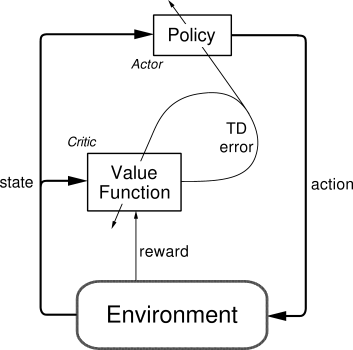
\includegraphics[width=.3\linewidth]{figures/actor_critic.png}
	        \caption{Actor-critic set-up. The actor (policy) receives a state from the environment and chooses an action to perform. At the same time, the critic (value function) receives the state and reward resulting from the previous interaction.~\parencite{arulkumaran2017brief}}
	        \label{fig:actor_critic}
\end{figure}


% \clearpage

\section{Deep Reinforcement Learning}

A recent breakthrough in deep learning fields relied on efficiently training a deep neural network on large training datasets, which improves many fields including \textit{computer vision and speech recognition}. These models are trained directly from raw inputs using stochastic gradient descent to update the networks' weights. These successes lead its way to reinforcement learning in which it connects RL algorithms with deep neural networks to operate directly on raw images and efficiently generate training data using stochastic gradient updates.

% \subsection{State of the Art}
In the following, we briefly discuss four state-of-the-art algorithms, \textit{Deep Q Network}, two deep policy search methods: \textit{Deep Deterministic Policy Gradient} and \textit{Proximal Policy Optimization}, also an asynchronous deep actor-critic method called \textit{Asynchronous Advanced Actor-Critic}.
These methods are currently the most popular and effective algorithms, proposed by DeepMind\footnote{\url{https://deepmind.com}} and OpenAI\footnote{\url{https://openai.com}}. In this work, some of these methods are used for experiments.

\subsubsection{Deep Q Network}
Deep Q Network (\textbf{DQN}) was first proposed by~\parencite{mnih2013playing}, it presents the first deep learning model to successfully learn control policies directly from high-dimensional sensory input using reinforcement learning.

Q-learning algorithm was used to make the decision, using stochastic gradient descent to update the weights. Since deep learning handles only with independent data samples, the \textit{experience replay} mechanism was used to break correlations along with \textit{Fixed Q-target}. DQN algorithm replaces the tabular representation for Q-value function with the deep neural network.

\subsubsection{Deep Deterministic Policy Gradient}
Since the rise of deep neural network function approximations for learning value or action-value function, deep deterministic policy gradient method have been proposed by~\parencite{lillicrap2015continuous}. It used an \textit{actor-critic} approach based on the \textbf{Deterministic Policy Gradient (DPG) algorithm}~\parencite{silver2014deterministic}, combined with \textit{experience replay and fixed Q-target} techniques which inspired by \textbf{DQN} to use such function approximation in a stable and robust way. In addition, a robust strategy in deep learning called \textit{batch normalization}~\parencite{ioffe2015batch} is adopted to scale the range of input vector observations in order to make the network capable of finding hyper-parameters which generalize across environments with different scales of state values.
The problem of exploration in off-policy algorithms like Deep Deterministic Policy Gradient (DDPG) can be addressed in a very easy way and independently from the learning algorithm. Exploration policy is then constructed by adding noise sampled from a noise process \textit{N} to the actor policy.

\subsubsection{Proximal Policy Optimization}
One of the main issues in policy gradient methods is defining the step size (\textit{learning rate $\alpha$}). Hence, the new robust policy gradient methods, which we call Proximal Policy Optimization (PPO)~\parencite{schulman2017proximal, heess2017emergence} was proposed to solve this problem. It also uses some of the benefits from trust region policy optimization~\parencite{schulman2015trust}. these methods bound parameter updates to a trust region to ensure stability. This algorithm is similar to natural policy gradient methods and it is also considered as a variant of Trust Region Policy Optimization (TRPO), it directly uses the first-order optimization methods to optimize the objective.

\subsubsection{Asynchronous Advanced Actor-Critic}
Asynchronous Advanced Actor Critic (A3C)~\parencite{mnih2016asynchronous} is an asynchronous method using Advanced Actor-Critic (A2C). \textit{\textbf{Asynchronous}} means asynchronously execute multiple agents in parallel, on multiple instances of the environment and all using a replica of the   (NN) (\textit{asynchronous data parallelism}). It often works in a multi-core CPU or GPU. The idea behind it is that there is a \textit{global network} and \textit{multiple actor-learners} which have their own set of network parameters. A thread is dedicated for each agent, and each thread interacts with its own copy of the environment.
Giving each thread a different exploration policy also improves robustness, since the overall experience available for training becomes more diverse. Moreover, in A3C just one deep neural network is used both for estimation of policy $\pi(s)$ and value function $V_{\pi}(s)$; because we optimize both of these goals together, we learn much faster and effectively. We also don’t need to consider the data correlation and oscillations issues because different agent gets different transitions when playing in the same environments.

% !TeX root = ../../main.tex

\section{Related Work}\label{related_work}

Recently, there have been multiple efforts and to scale up deep reinforcement learning, starting with methods that rely on distributed asynchronous stochastic gradient descent (SGD)~\parencite{dean2012large} with multiple workers. They developed a software framework called \textbf{DistBelief} that can utilize computing clusters with thousands of machines to train large models. It consists of two main ingredients shown in the Figure~\ref{fig:sgd} below. First, the parameters of the model can be distributed on multiple servers, depending on the architecture. This set of servers are called the \textit{parameter servers}. Second, there can be multiple workers processing data in parallel and communicating with the parameter servers. Since each worker communicates with the parameter servers independently of the others, this is called \textit{Asynchronous Stochastic Gradient Descent} (Async-SGD).

In practice, it means that while a worker computes gradients of the loss with respect to its parameters on a given mini-batch, other workers also interact with the parameter servers and thus potentially update its parameters, hence when a worker sends back its gradients to the parameter server, these gradients are usually computed w.r.t. the parameters of an old version of the model. When a model is trained with N workers, each update will be $N-1$ steps old on average.

\begin{figure}[!htb]
	\centering
	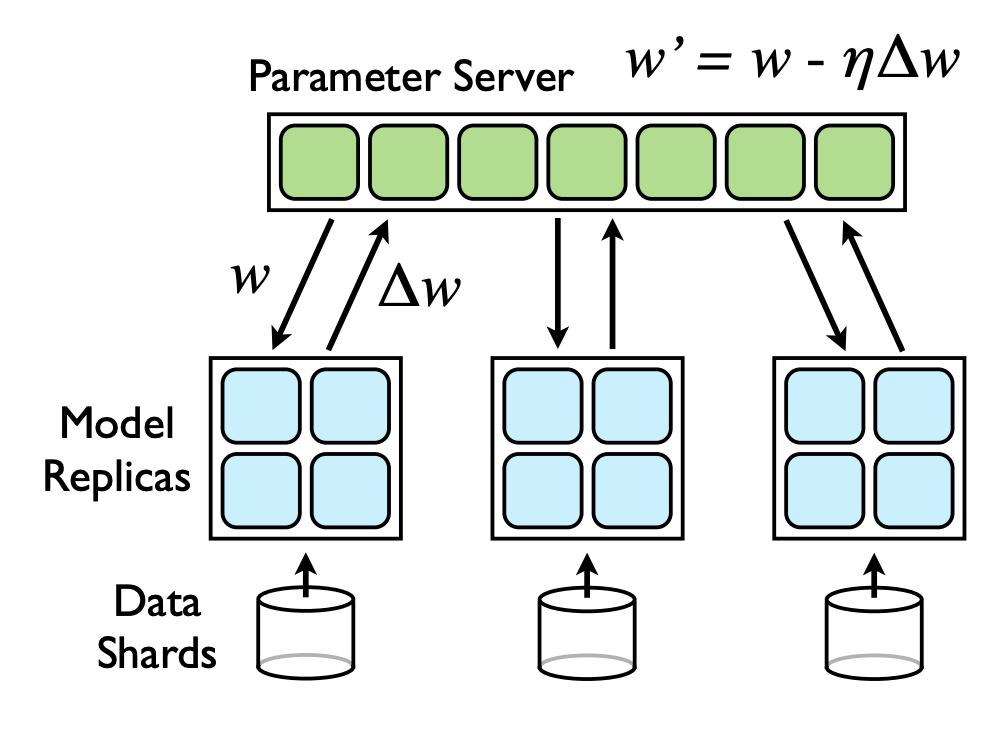
\includegraphics[width=0.5\linewidth]{figures/algos/sgd.png}
	\caption{Async-SGD~\parencite{dean2012large}: Model replicas asynchronously fetch parameters w and push gradients \(\Delta w\) to the parameter server.}
	\label{fig:sgd}
\end{figure}


Since the development of Async-SGD~\parencite{dean2012large}, a couple of different RL algorithms have proposed. Some algorithms have followed the approaches introduced in the paper. Others have introduced distribution for experience replay buffers and follow the parallel learners and actors approach to generate new behaviors and store experiences that get collected. In the following, a description for the most successful algorithms which rely on a distributed setup:

$\bullet$ \textit{\textbf{A distributed version of Deep Q-Networks}}~\parencite{ong2015distributed} where they adapt the \textit{DistBelief} software framework to the context of efficiently training reinforcement learning agents to distribute the deep Q-network training. resulting the method is completely asynchronous and scales well with the number of machines.

$\bullet$ \textit{\textbf{Massively parallel methods for DRL (Gorila)}}~\parencite{nair2015massively}, which uses a distributed experience replay buffer (and no prioritization). This architecture shown in Figure~\ref{fig:gorila_arch} uses four main components: \textit{parallel actors} that generate new behaviour, \textit{parallel learners} that are trained from stored experience, \textit{a distributed neural network} to represent the value function or behaviour policy, and \textit{a distributed store of experience} with no prioritization. It was applied to \textbf{49 games} from Atari 2600 games from the Arcade Learning Environment (ALE), using identical hyperparameters. The performance shown in Figure~\ref{fig:gorila_results} surpassed \textit{non-distributed DQN} in \textbf{41} of the 49 games and also reduced the wall-time required to achieve these results by an order of magnitude on most games.

\begin{figure}[!htb]
	\centering
	\begin{subfigure}[b]{0.4\textwidth}
		\centering
		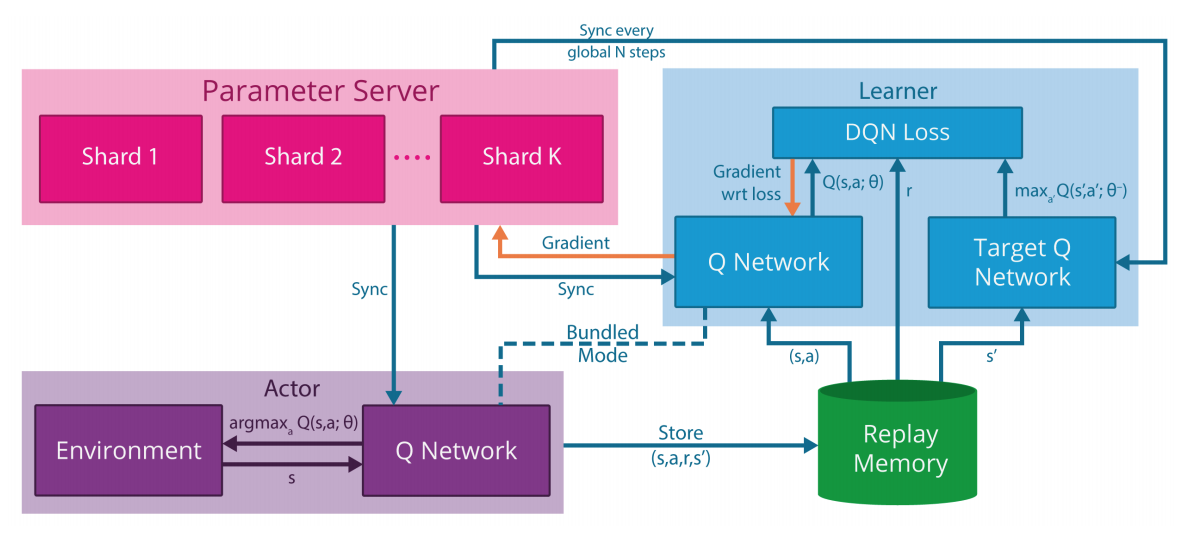
\includegraphics[width=\textwidth]{figures/algos/gorila.png}
		\caption{Agent parallelizes the training procedure by separating out learners, actors and parameter server}
		\label{fig:gorila_arch}
	\end{subfigure}
	\hfill
	\begin{subfigure}[b]{0.4\textwidth}
		\centering
		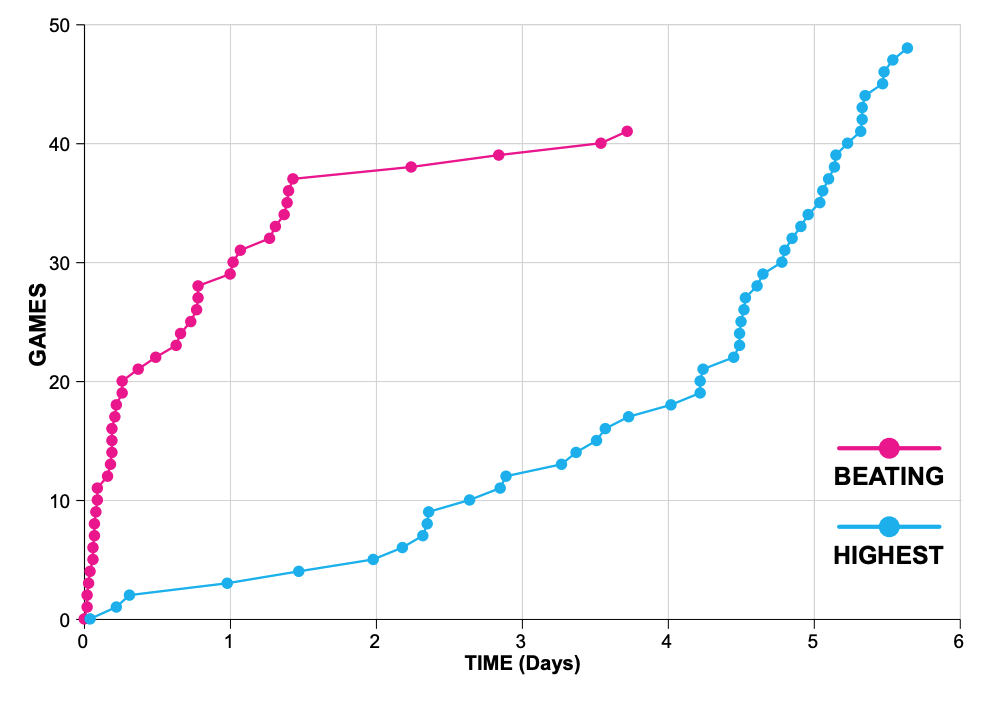
\includegraphics[width=\textwidth]{figures/algos/gorila_results.png}
		\caption{Red curve: time to surpass single DQN\\
		Blue curve: time to reach its peak performance}
		\label{fig:gorila_results}
	\end{subfigure}
	\hfill
	\caption{The Gorila Architecture \& Results | Figures from Gorila paper~\parencite{nair2015massively}}
	\label{fig:gorila}
\end{figure}

$\bullet$ \textit{\textbf{Asynchronous methods for DRL (A3C)}}~\parencite{mnih2016asynchronous}, in which they present asynchronous variants of four standard reinforcement learning algorithms and show that parallel actor-learners have a stabilizing effect on training allowing all four methods to successfully train neural network controllers using asynchronous gradient descent for optimization. The algorithm shown in Figure~\ref{fig:a3c_workflow} used multiple threads to run copies of the environment and generate uncorrelated sequences of training samples. Parameters were then sent to a shared parameter server at regular intervals. Because this promotes non-stationarity for the sequences of SARSA tuples, experience replay is not necessarily needed. The implementations of gradient-based optimization technique (RMSProp) and Momentum SGD used by the authors employed a Hogwild-inpsired~\parencite{recht2011hogwild} lock-free scheme for maximum efficiency. A3C is the ``best'' agent that was presented in this paper. It is an asynchronous advantage actor-critic algorithm as shown in Figure~\ref{fig:a3c_arch}. It maintains an approximation of the policy, an estimate of the value function, and computes an ``advantage'' function and a variance-reducing baseline~\parencite{degris2012off}. An entropy regularization term was also used to discourage premature convergence. The A3C performance overpassed gorila and add some enhancement including faster updates, removing  the replay buffer, and moving to Actor-Critic (from Q learning).

The State of the art results in Figure~\ref{fig:a3c_results} were obtained on some of the Atari games (ALE). An LSTM-based A3C agent was tested with Deepmind’s Labyrinth environment. They also tested on the TORCS car racing environment and MuJoCo, the continuous-space physics simulation engine.

\begin{figure}[!htb]%{0.5\textwidth}
	\centering
	\begin{subfigure}[b]{0.33\textwidth}
		\centering
		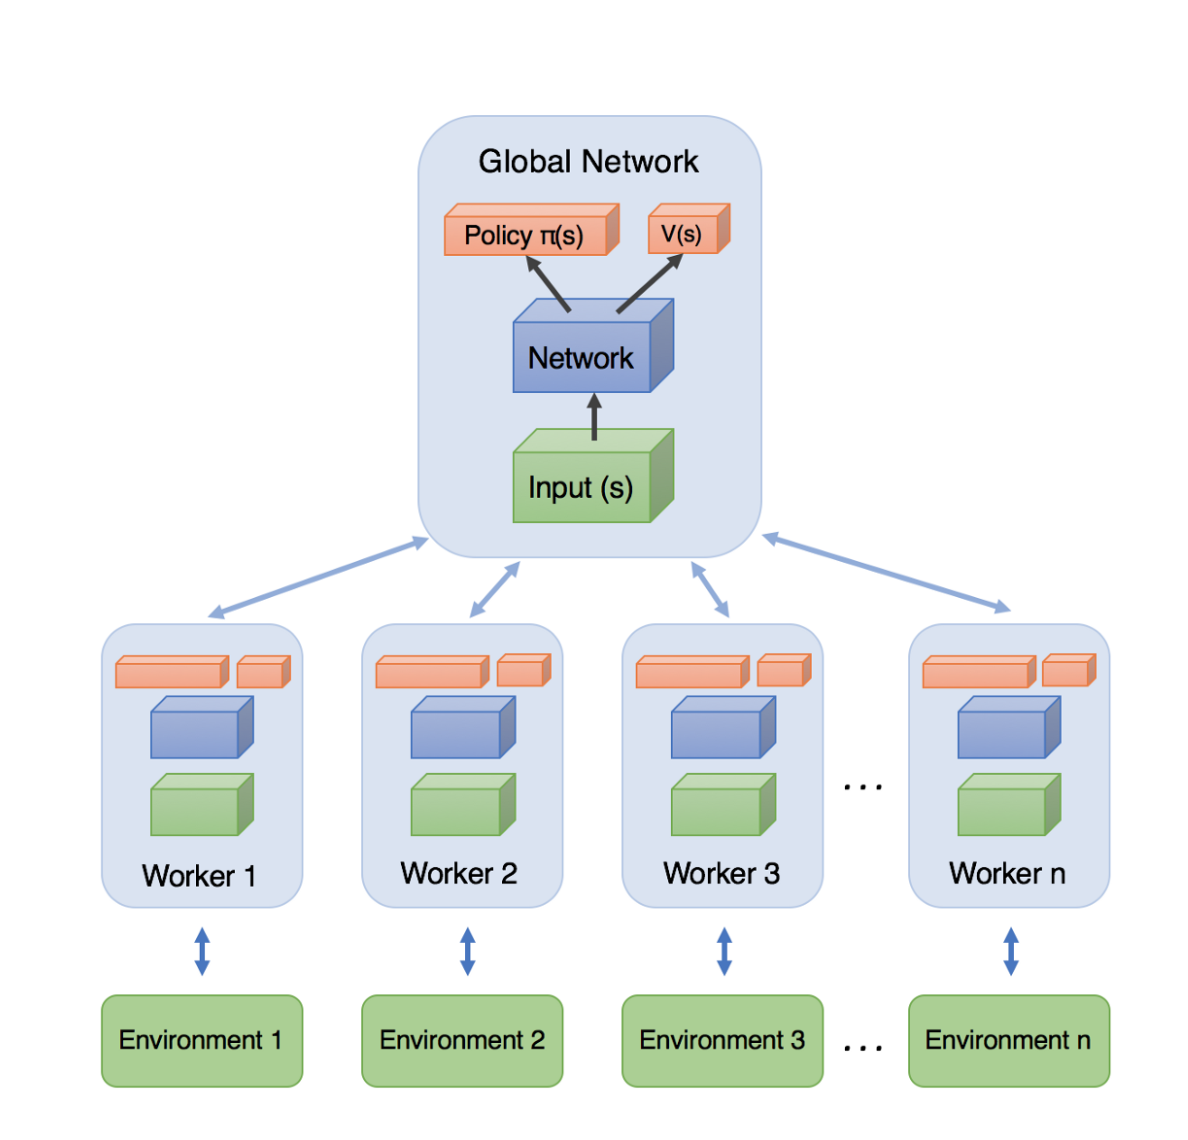
\includegraphics[width=\textwidth]{figures/algos/a3c.png}
		\caption{A3C high-level architecture.}
		\label{fig:a3c_arch}
	\end{subfigure}
	\hfill
	\begin{subfigure}[b]{0.33\textwidth}
		\centering
		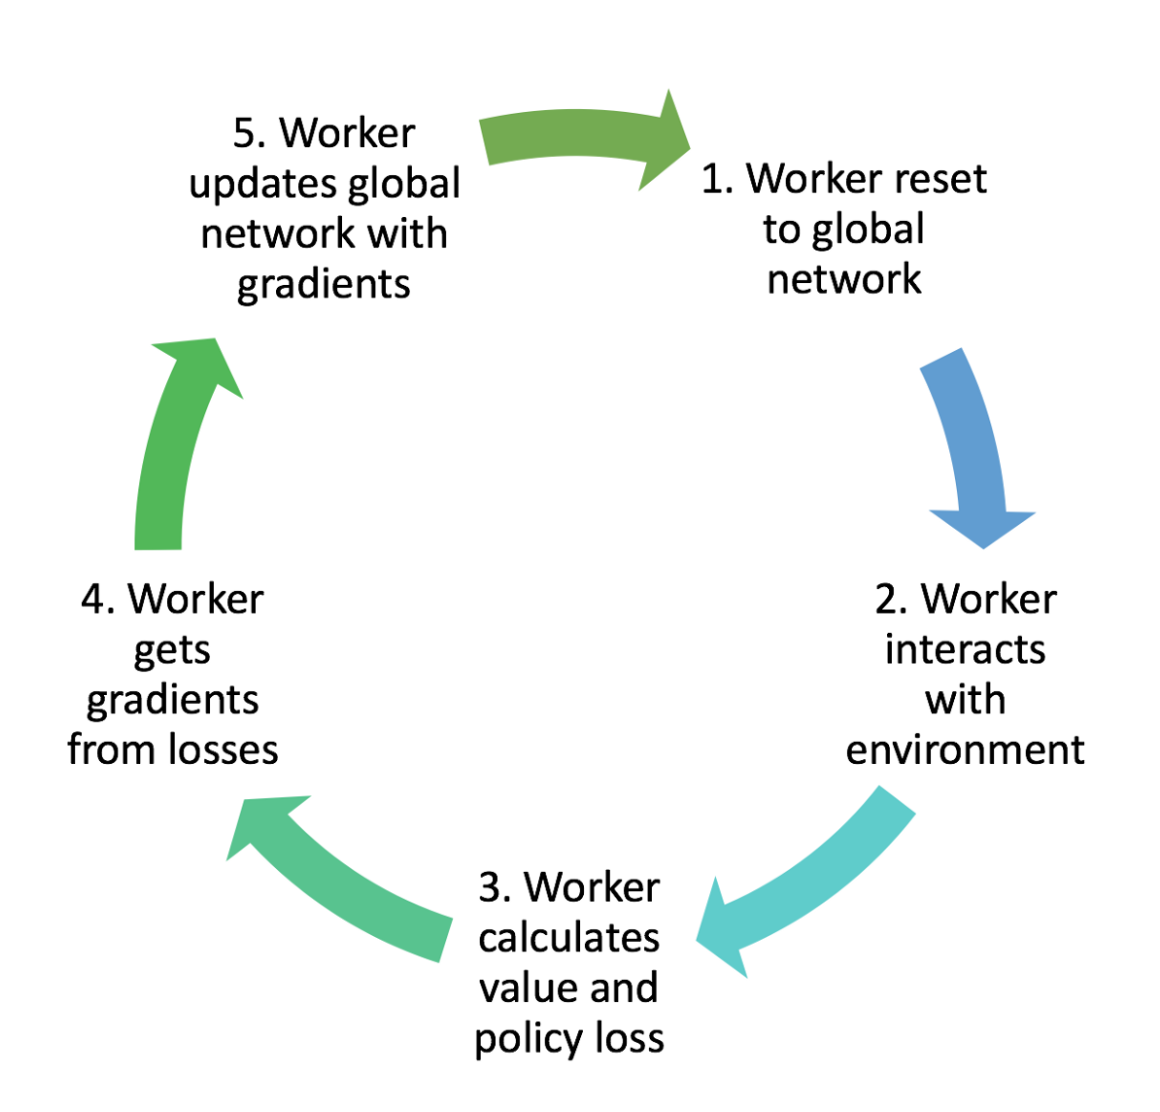
\includegraphics[width=\textwidth]{figures/algos/a3c_workflow.png}
		\caption{Training workflow of each worker agent in A3C.}
		\label{fig:a3c_workflow}
	\end{subfigure}
	\hfill
	\begin{subfigure}[b]{0.33\textwidth}
		\centering
		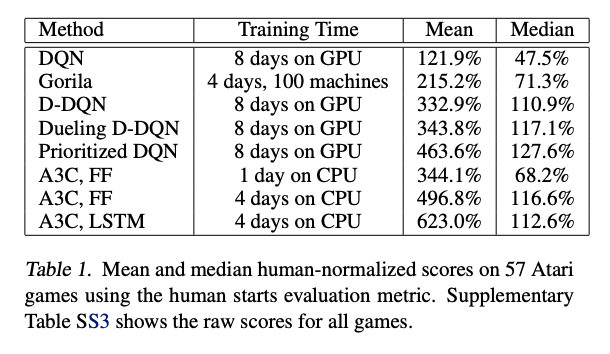
\includegraphics[width=\textwidth]{figures/algos/a3c_results.png}
		\caption{A3C Results}
		\label{fig:a3c_results}
	\end{subfigure}
	\hfill
	\caption{The A3C Architecture, workflow \& Results | Figures from A3C paper~\parencite{mnih2016asynchronous}}
	\label{fig:a3c}
\end{figure}

Another direction with some alternatives to \textit{asynchronous SGD} methods which includes distributed BA3C~\parencite{adamski2018distributed}, Evolution strategies~\parencite{salimans2017evolution} using evolutionary processes and 

$\bullet$ \textit{\textbf{Distributed Prioritized Experience Replay (Ape-X)}} which use a distributed replay with synchronous learner. They focused on applying the Ape-X framework to DQN and DPG. Also it could be combined with any other off-policy reinforcement learning update. 

The main idea of Ape-X paper~\parencite{horgan2018distributed} is to scale up the experience replay data by having many actors running in parallel collect samples of experience. The actors periodically pool their samples into a centralized data repository, which is used for experience replay for a centralized learner to select from it in a prioritized fashion~\parencite{schaul2015prioritized} and update neural network parameters as shown in Figure~\ref{fig:apex_arch}. Those parameters then get copied back to the actors. Due to the distributed prioritization, experience collection can scale to hundreds of CPU workers. Hence, they step over and complement standard distributed training approaches~\parencite{dean2012large} of neural networks which focus on parallelizing the computation of gradients to \textit{distribute the generation and selection of experience data}, which suffices to improve results. 

This high-throughput architecture achieved state of the art results, as shown in~\ref{fig:apex_results}, in a wide range of discrete and continuous tasks, both in terms of wall-clock learning speed and final performance.

\begin{figure}[!htb]
	\centering
	\begin{subfigure}[b]{0.5\textwidth}
		\centering
		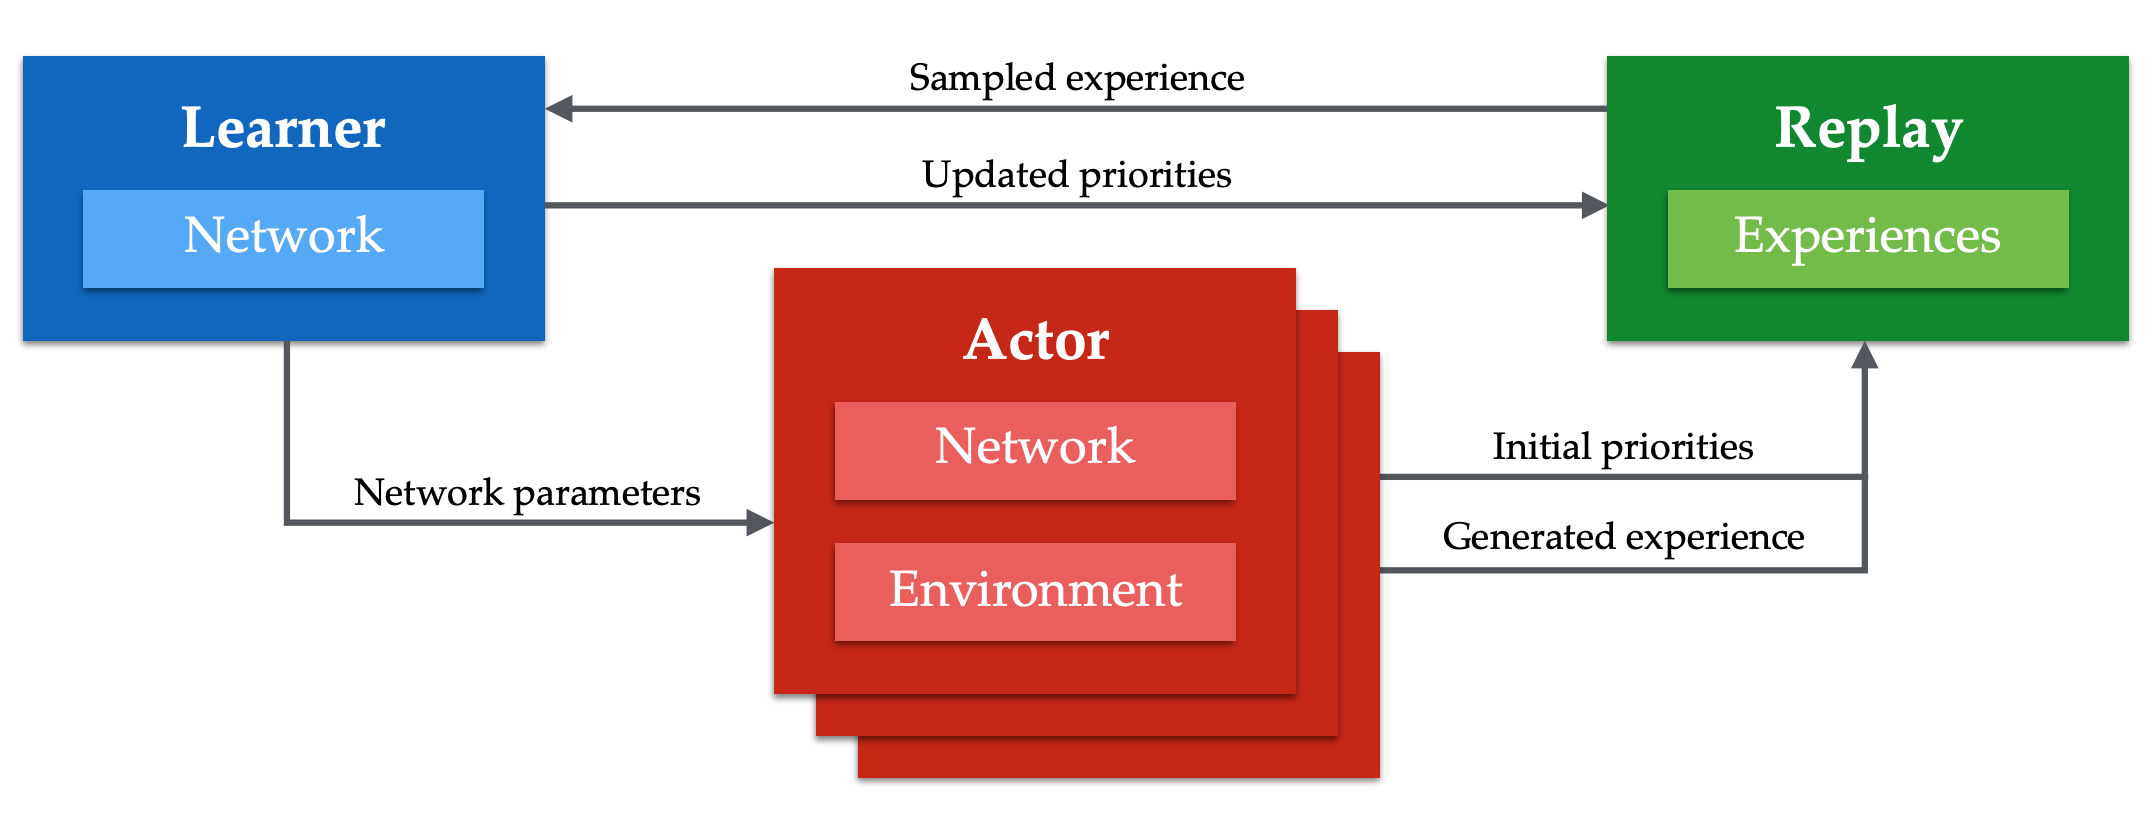
\includegraphics[width=\textwidth]{figures/algos/apex.png}
		\caption{The Ape-X architecture}
		\label{fig:apex_arch}
	\end{subfigure}
	% \hfill
	\begin{subfigure}[b]{0.5\textwidth}
		\centering
		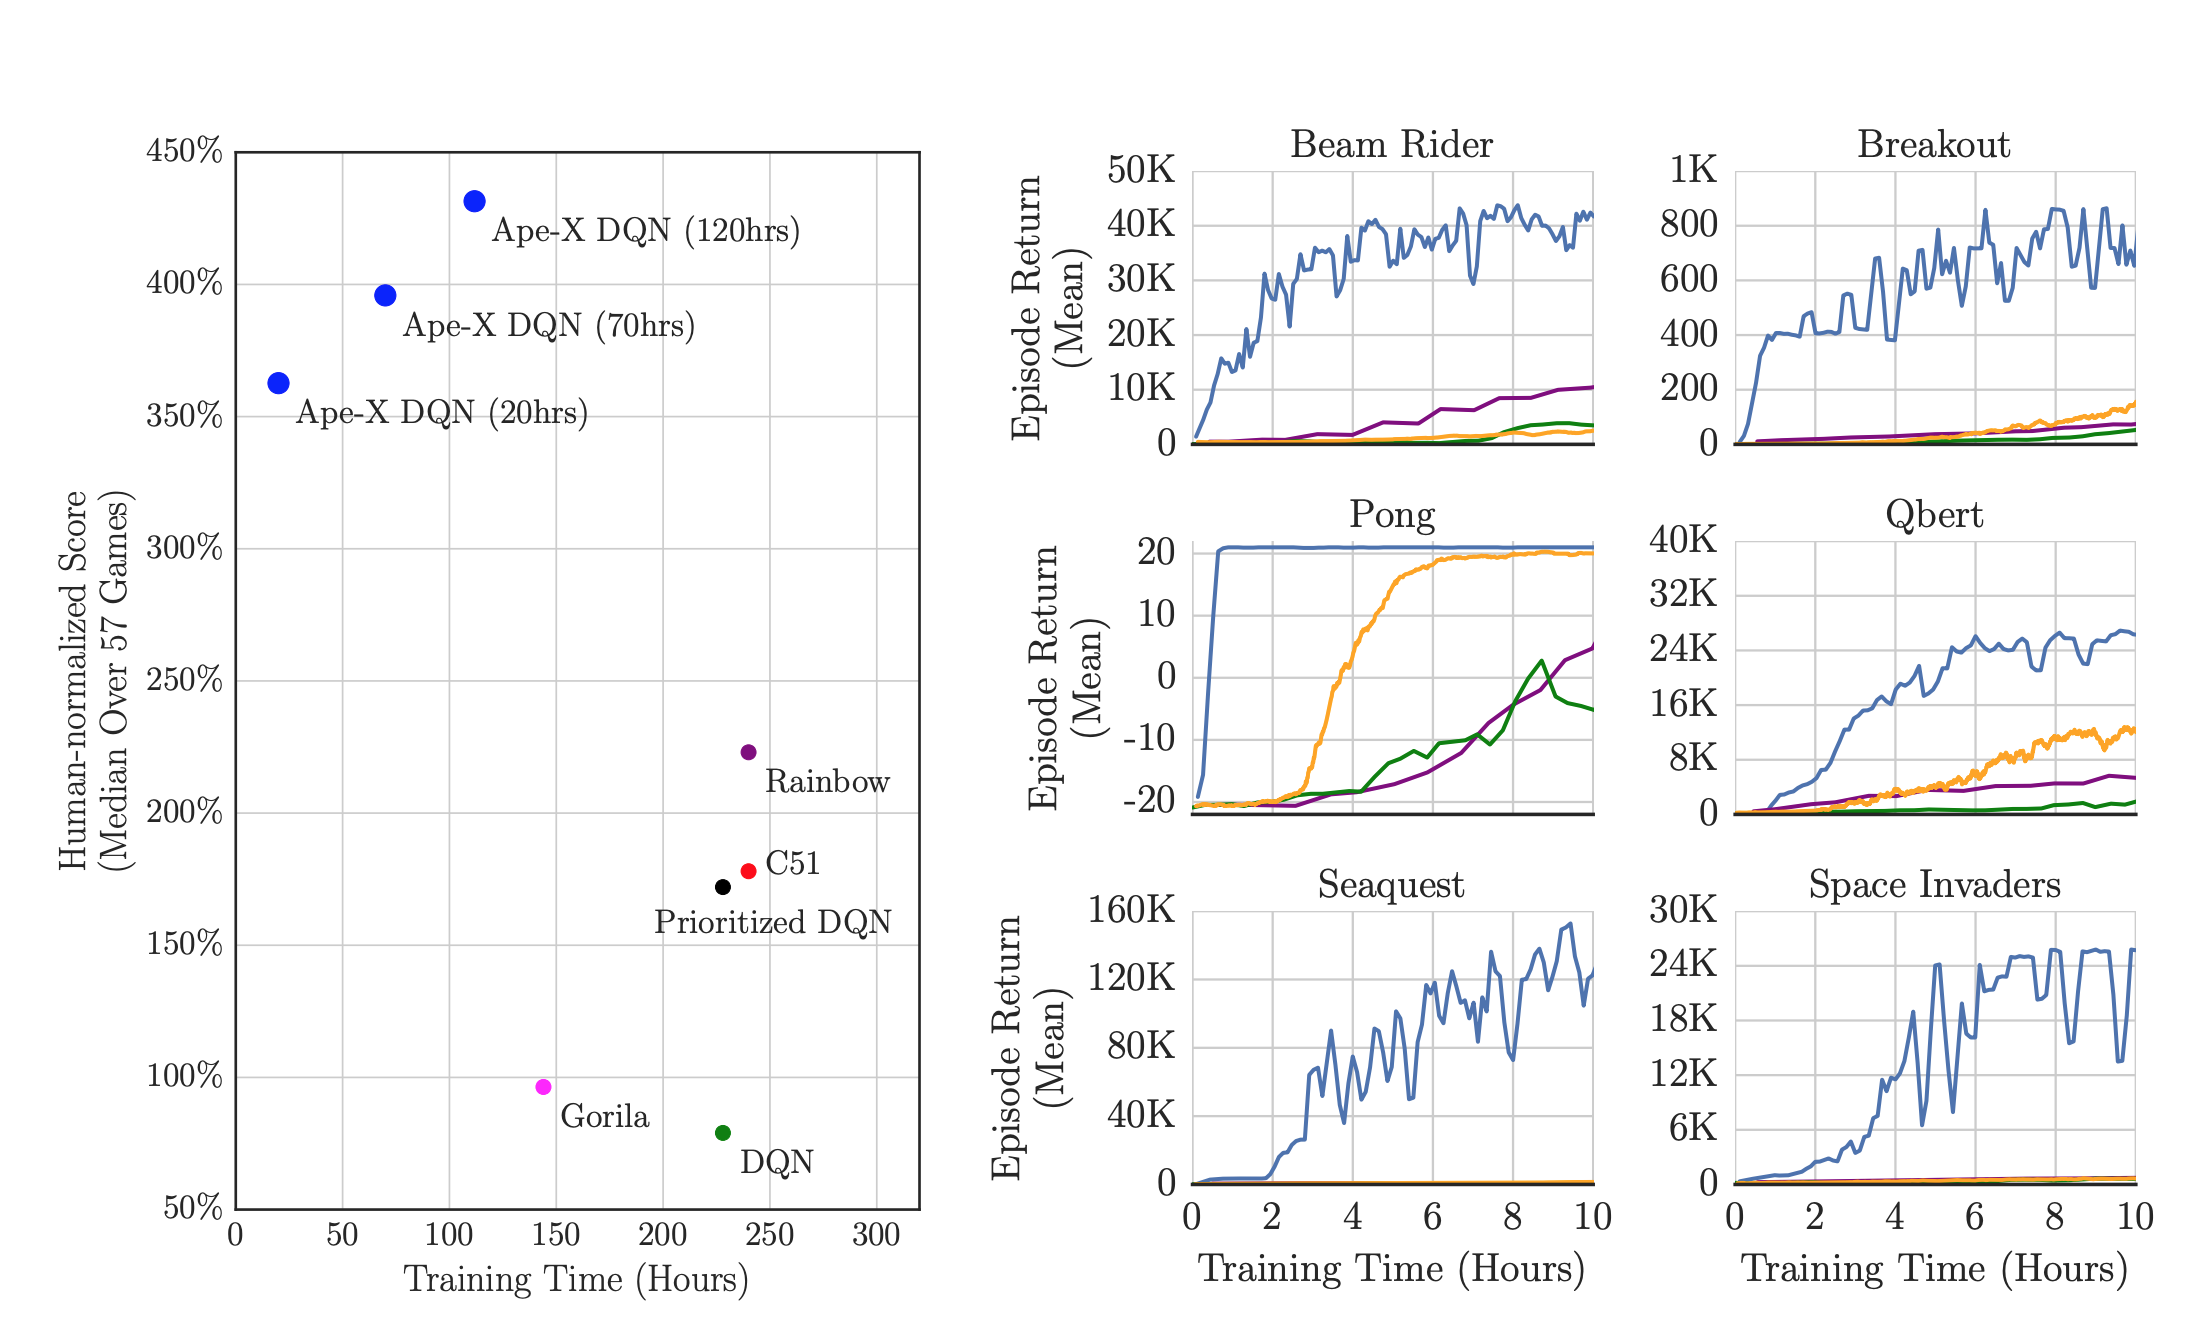
\includegraphics[width=\textwidth]{figures/algos/apex_results.png}
		\caption{Ape-X Performance compared with other RL algorithms}
		\label{fig:apex_results}
	\end{subfigure}
	\hfill
	\caption{The Ape-X Architecture \& Results | Figures from Ape-X paper~\parencite{horgan2018distributed}}
	\label{fig:apex}
\end{figure}

Other research has attempted to scale up by using multiple GPUs and utilizing them. The simplest method is batched A2C~\parencite{clemente2017efficient} in which with every step produces a batch of actions and applies them to a batch of environments. BA3C~\parencite{babaeizadeh2016ga3c} another method which uses asynchronous data collection to effectively utilize GPUs.

The most recent work done in the are of distributed DRL and multi-tasking learning which achieve the state of the art performance is \textit{Importance Weighted Actor-Learner Architectures} \textbf{(IMPALA)}~\parencite{espeholt2018impala} by DeepMind. It is a scalable distributed DRL algorithm for their newly designed DMLab-30 environment (which is a collection of new levels designed using our open-source RL environment \textit{DeepMind Lab}). These environments are provided to test systems on a large spectrum of interesting tasks either individually or in a multi-task setting)

Importance Weighted Actor-Learner Architecture, appeared in~\ref{fig:impala_arch}, is inspired by the popular \textbf{A3C} architecture which uses multiple distributed actors to learn the agent’s parameters. The developed new distributed agent impala maximizes data throughput using an efficient distributed architecture with TensorFlow. 
In the training process for actor-critic methods, each of the actors uses a clone of the policy parameters to act in the environment. Periodically, actors pause their exploration to share the gradients they have computed with a central parameter server that applies updates. 

\begin{figure}[!htb]
	\centering
	\begin{subfigure}[b]{0.45\textwidth}
		\centering
		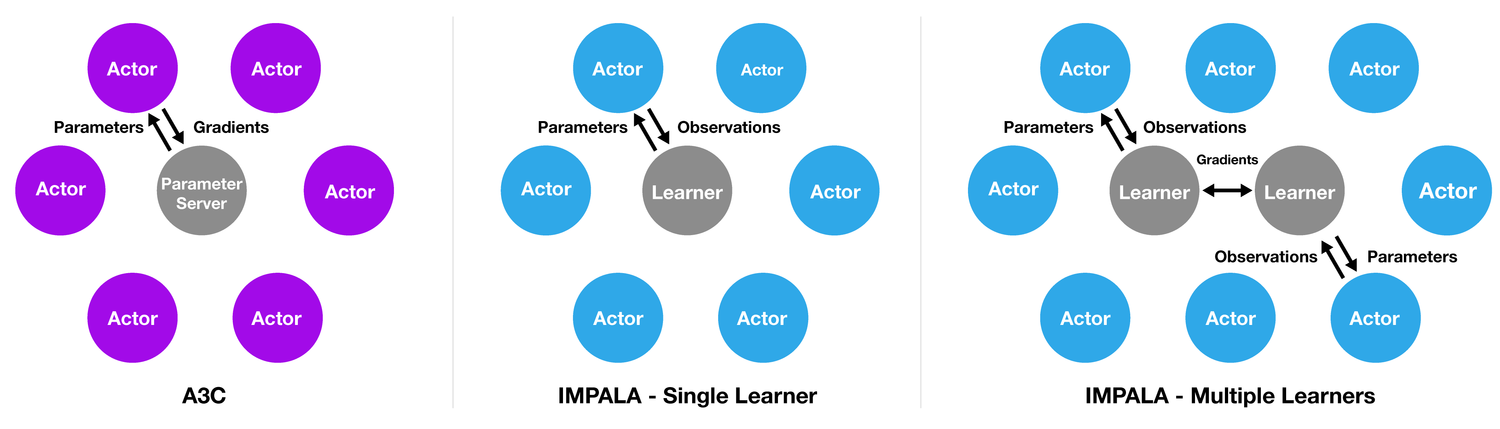
\includegraphics[width=\textwidth]{figures/algos/impala.png}
		\caption{The IMPALA Architecture.}
		\label{fig:impala_arch}
	\end{subfigure}
	\hfill
	\begin{subfigure}[b]{0.45\textwidth}
		\centering
		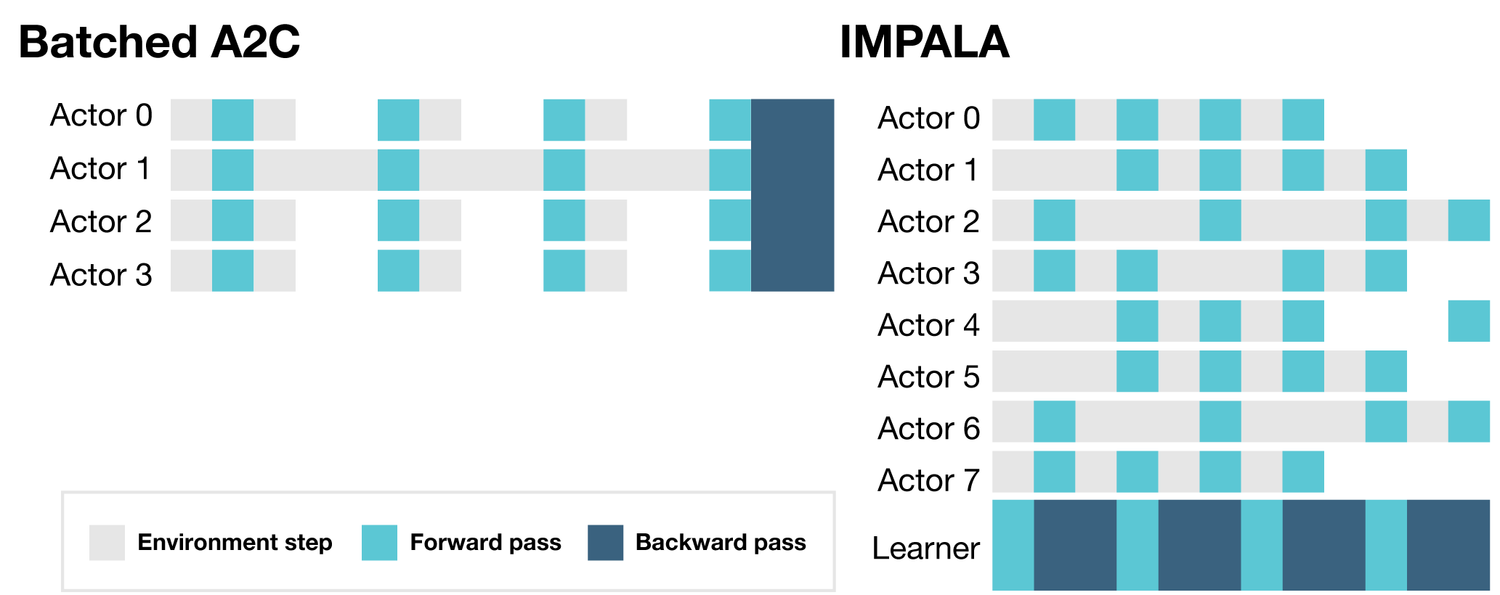
\includegraphics[width=\textwidth]{figures/algos/impala_vs_a2c.png}
		\caption{IMPALA vs Batched A2C Training}
		\label{fig:impala_vs_a2c}
	\end{subfigure}
	\hfill

	\begin{subfigure}[b]{0.45\textwidth}
		\centering
		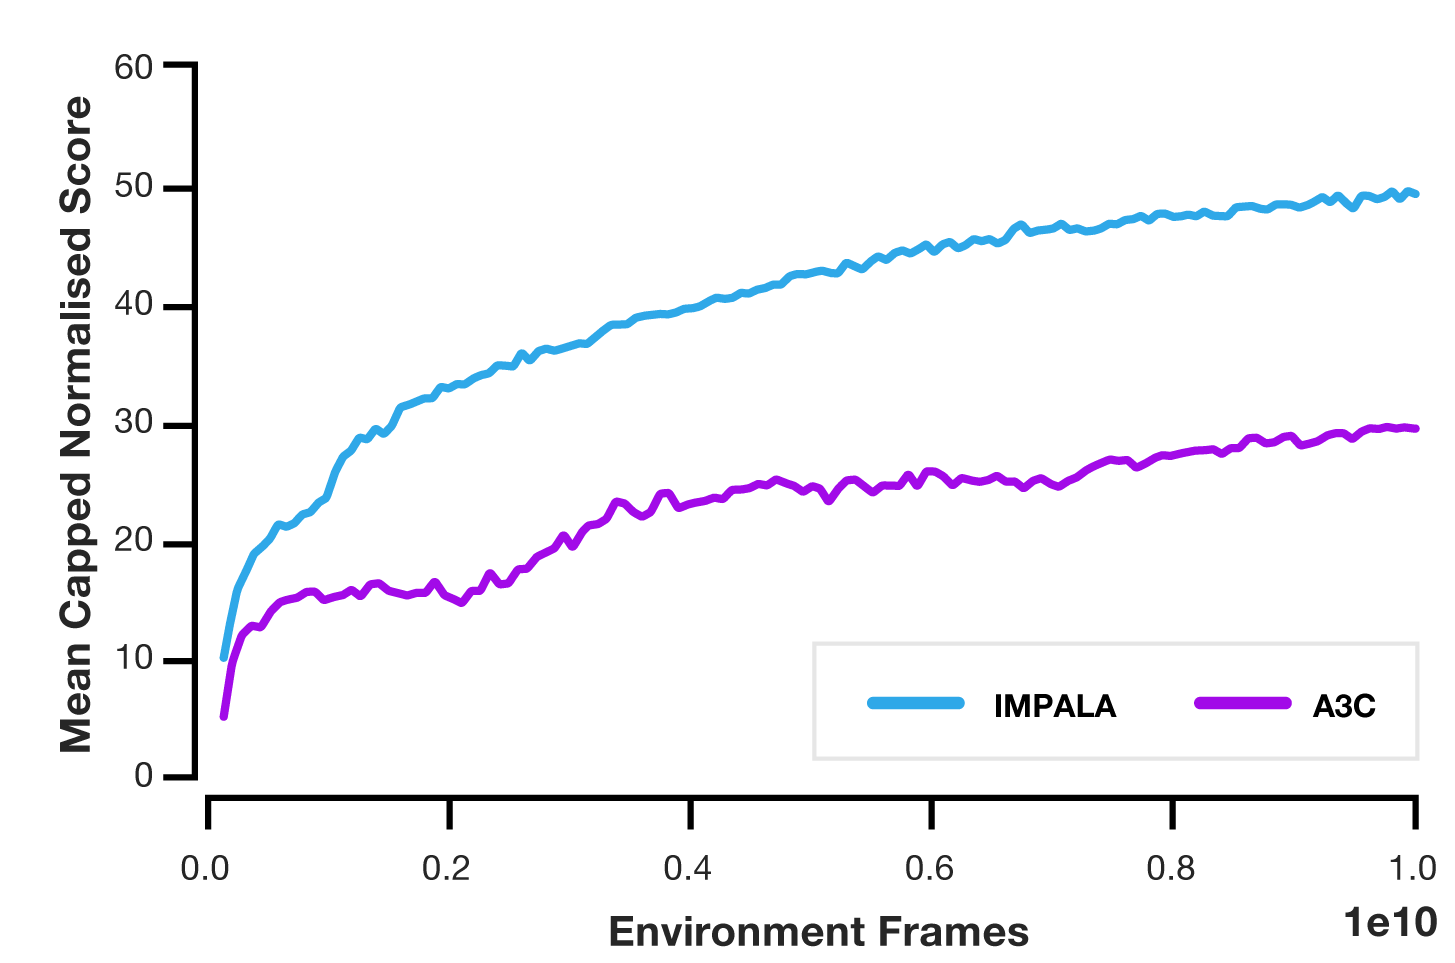
\includegraphics[width=\textwidth]{figures/algos/impala_results.png}
		\caption{IMPALA Results}
		\label{fig:impala_results}
	\end{subfigure}
	\hfill
	\caption{The IMPALA Architecture, Comparison \& Results | Figures from IMPALA paper~\parencite{espeholt2018impala}}
	\label{fig:impala}
\end{figure}



On the other hand, impala's actors are not used to calculate gradients. Instead, they are just used to \textit{collect experience} which is passed to a \textit{\textbf{central learner}} that computes gradients, resulting in a model that has completely independent actors and learners. Separating the learning and acting in this way also has the advantage of increasing the throughput of the whole system since the actors no longer need to wait for the learning step like in architectures such as batched A2C as shown in Figure~\ref{fig:impala_vs_a2c} above. This allows us to train impala architectures on interesting environments without suffering from variance in frame rendering-time or time-consuming task restarts.

However, decoupling the acting and learning causes the policy in the actor to lag behind the learner. To compensate for this difference we introduce a principled off-policy advantage actor-critic formulation called V-trace which compensates for the trajectories obtained by actors being off policy. Importance Weighted Actor-Learner Architecture was \textbf{10 times} more data-efficient and achieved double the final score compared to distributed A3C as shown in the Figure~\ref{fig:impala_results} above. Moreover, Importance Weighted Actor-Learner Architectures showed positive transfer from training in multi-task settings compared to training in the single-task setting.


On the practical side, there have been some frameworks developments that focus on distributed deep reinforcement learning and applying all the techniques and algorithms to multiple environments for the sake of advancing DRL research. Dopamine~\parencite{castro2018dopamine} is a new framework for flexible and reproducible RL Research by Google in which they provide large-scale distributed training and enabling distributing the learning process across multiple workers. Using distributional methods that allow agents to model full distributions, rather than simply their expected values, to learn a more complete picture of their world. This framework aims to provide flexibility, stability, and reproducibility for new and experienced RL researchers alike. 

Ray~\parencite{moritz2018ray} is another more general framework with distributed execution for AI applications. Ray is a high-performance distributed execution framework targeted at large-scale machine learning and reinforcement learning applications. It achieves scalability and fault tolerance by abstracting the control state of the system in a global control store and keeping all other components stateless. It uses a shared-memory distributed object store to efficiently handle large data through shared memory, and it uses a bottom-up hierarchical scheduling architecture to achieve low-latency and high-throughput scheduling. It uses a lightweight application programming interface (API) based on dynamic task graphs and actors to express a wide range of applications in a flexible manner.